\chapter{Intro to virus}
\label{cha:6}
%\documentclass[10pt]{article}\

%%%%%%%%%%%%%%%%%%%%%%%%%%%%%%%%%%%%%%%%%%%%%%%%%%%%%%%%%%
%%%%%			Introduction Chapter 6			%%%%%%
%%%%%												%%%%%%
%%%%%												%%%%%%
%%%%%%%%%%%%%%%%%%%%%%%%%%%%%%%%%%%%%%%%%%%%%%%%%%%%%%%%%%


\section{Introduction}
This section gives a formal definition of the FlipIt game with a virus propagation. First we derive a formula for a FlipIt game without a virus. After that we introduce a modification to this formula to achieve an adapted formula for a FlipIt game with a virus propagation. 
%In this section we are going to elaborate how we are going to model a Flipit game with multiple resources and a virus that propagates and infects the resources. We come up with a formula for the normal FlipIt (normal as in specific parameters and no normalising over the first interval) and then reform it to a FlipIt game with a virus. 

\subsection{FlipIt with a virus propagation}
In the previous section the FlipIt game is already been explained. In this section we will introduce a FlipIt game with a virus propagation. A FlipIt game with a virus propagation is a game where the attacker will drop a virus on one of the resources that is available. The virus will then spread itself to the neighbour resources. The attacker will only gain control over the whole network, in general the game, when it has infected all the resources. All the resources will not be infected immediately when the attacker has dropped its virus. It will take some time before the virus is spread and has infected everything. The time that it takes for the virus to infect every resource will be denoted as parameter \textit{d}. If we want to measure how long it takes for the virus to infect all resources, we have to calculate the shortest path to the farthest node. This can be measured by a method that we will explain in section []. With this parameter we can compose a formula to calculate the gain of a FlipIt game with a virus propagation.  \\ \todo{uitleggen waarom we een gewone flippit kunnen nemen met 1 resource}

The gain of a player is defined as the total amount of time that a player has owned the resource over the amount of time that has passed since the beginning of the game. If the attacker attacks with the virus it will cause a delay of length \textit{d}. This means that the gain of the player from the normal game has to be abstracted with a delay everytime the attacker moves. This game, where the attacker drops a virus, cannot be modelled completely by a FlipIt game with a delay. This is because if the delay is bigger than the period of the attacker, the attacker will gain no control. If it would be with the delay caused by a phase bigger than zero the attacker would gain control after the defender flipt again. This is explained in figure \ref{fig:virusflip}. In the next section a formal definition 

\subsection{chap}
The setting of the game that we are going to play is one with multiple resources. When the defender flips it will always flip all the resources. The attacker will flip the node in the graph that can infect all the nodes in the shortest time possible. The attacker will gain the control over the resources when all the resources are infected. So ''d'' will be the shortest path to the furthest node. We will model ''d'' in time units. \todo{moet misschien niet ? }.
\begin{figure}[hbtp]
\caption{Difference in a FlipIt game between delay caused by a virus and a phase bigger than zero for the Attacker}
\centering
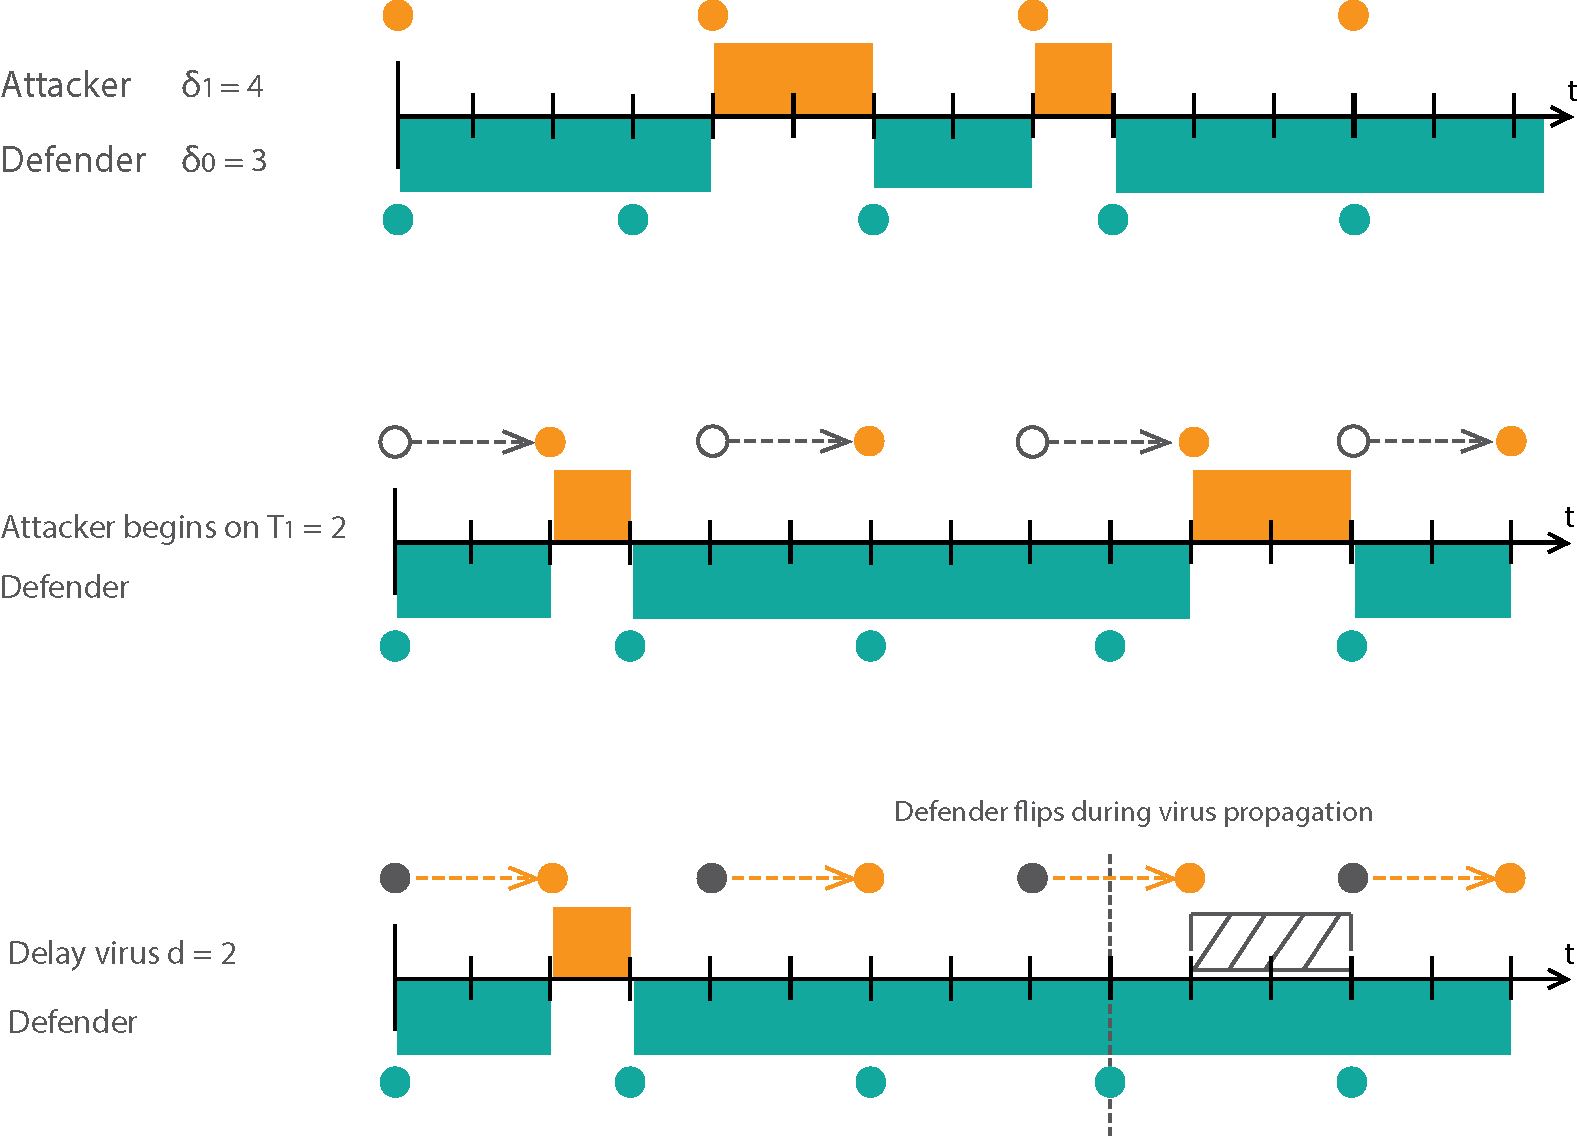
\includegraphics[scale=1]{Images/Flipvirus}
\label{fig:virusflip}
\end{figure}




\subsection{define formula}
Their is a definition given by the writers of the paper FlipIt, but we want to add the property of a virus to the game so we are trying to find a formula that defines a game by counting the amount of time one of the players has control. \\
\begin{figure}[hbtp]
\caption{Defining unit of control}
\centering
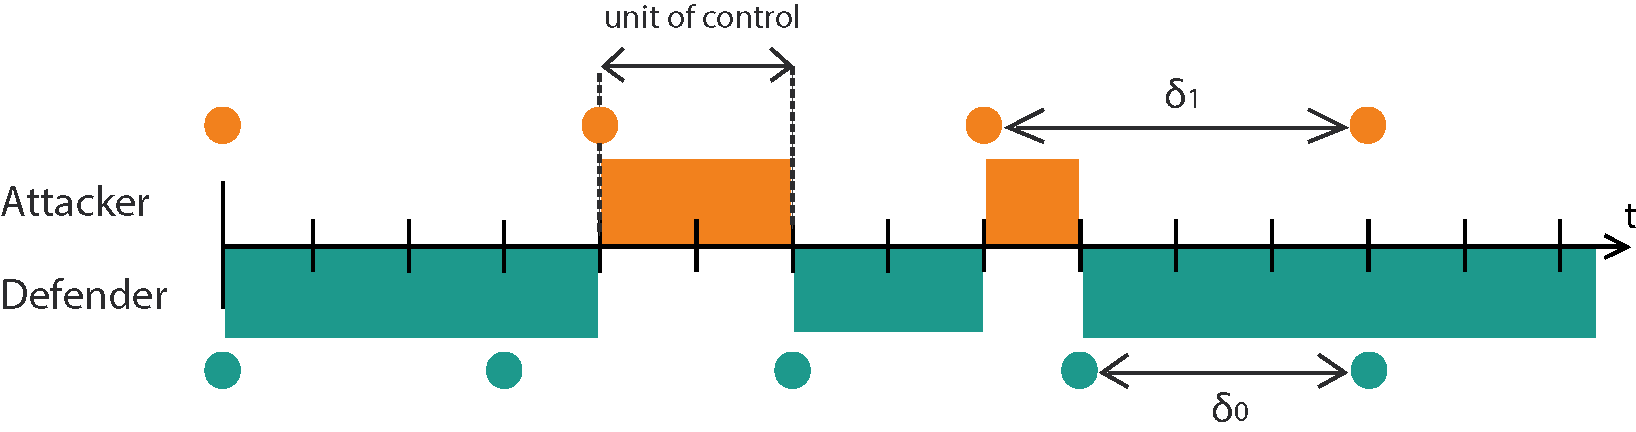
\includegraphics[scale=1]{Images/FlipSpel.png}
\end{figure}


%\begin{equation}\label{first}
%n = \delta_{1} mod \delta_{0}
%\end{equation}
%
%\begin{equation}\label{first}
%\Delta A = [( \delta_{0} - n + 1 ) * \delta_{1}] mod \delta_{1}
%\end{equation}
%
%\begin{equation}\label{first}
%\sum_{i=0}^{\delta_{1}} \lbrace [( \delta_{0} - i + 1 ) * \delta_{1}] mod \delta_{1} \rbrace
%\end{equation}
%\todo{formule met i nakijken}


for $delta_{1} > delta_{0}$ (The defender moves faster than the attacker.) \\

We will call every continuous time step that one of the players has control over the resource a unit of control. 
Next we will divide our time line of our FlipIt game into different intervals of size $delta_{1}$. So every time the attacker takes control we have the start of a new interval. Because the defender will move faster than the attacker it will at least move 1 time during the interval. Because the attacker only moves at the start of the interval we can say that the defender will always end as being in control of the resource. This brings us to the next forumula to calculate the length of a unit of control of the attacker. 
For every real number $delta_{1}$ and $delta_{0}$ and every n $\in$ of the natural numbers:
\begin{equation}\label{first}
\Delta A = [( 1- n  ) \times \delta_{1}] mod \delta_{0}
\end{equation}
where n is the number of the unit of control that you want to calculate of the attacker.\\

In this formula we multiply the number of unit of control that we want with the period of Attacker ( $\delta_{1}$). The 1 - n is when we count beginning from 1. If we start counting starting at 0 we leave the 1 and the formula becomes:
\begin{equation}\label{first}
\Delta A = [( - n  ) \times \delta_{1}] mod \delta_{0}
\end{equation}

We know that each interval ends with the control for the defender. This means that we only need to know how long the defender had control during that interval and take the rest. The rest will be the amount of time the attacker has control in that interval. We take the rest by doing the $mod \delta_{0} $

This means that if we want to calculate the gain of the attacker we need to calculate the time the attacker has control over the total amount of time that has passed by.
For $\delta_{0}$ and $\delta_{1}$ $\in$ Rational numbers we can see that we have a cycle. A pattern that comes back over and over again. That is when the amount of time is a multiple of $\delta_{0}$ and $\delta_{1}$ or the largest common multiplier (lcm). At this point the Attacker and the Defender move at the same time what brings us back to the beginning.
So to calculate the gain of $\delta_{0}$ and $\delta_{1}$ $\in$ Rational numbers we need to calculate the amount of control units of the attacker that go into the length of time units equal to the lcm of  $\delta_{0}$ and $\delta_{1}$. After this calculation we divide it by the lcm of $\delta_{0} $ and $ \delta_{1}$, which is the total amount of time and the amount of time for one cycle.  This gives us the following formula:
\begin{equation}\label{first}
a = \dfrac{\delta_{0} }{lcm(\delta_{0},\delta_{1})} 
\end{equation}
\begin{equation}\label{first}
\dfrac{\sum_{i=0}^{a} \lbrace [( 1 - i ) \times \delta_{1}] mod \delta_{0} \rbrace \rbrace }{lcm(\delta_{0},\delta_{1})} 
\end{equation}

We can also define a formula without the greatest common divider. Every $\delta_{0}$ and $\delta_{1}$ have to be written in a fraction:
\begin{equation}\label{first}
\delta_{0}=\dfrac{a}{b} ~~~~and~~~~\delta_{1}=\dfrac{c}{d}
\end{equation}
If  $\delta_{0}$ or $\delta_{1}$ is a Geheel getal then b or d will be 1. The formula for the gain becomes different:\\

\todo{formule zoeken zonder lcm en gcd}


If $\delta_{0}$ and/or $\delta_{1}$ is an Irrational number:
An irrational number $ i \neq \dfrac{a}{b}$ with $b \in Z, a \in N$
Because we cannot write \textit{i} in a fraction, this means that we won't have a cycle. If we would have a cycle that means that we do have a number that divides \textit{i}. If we don't have a cycle it goes on forever. Meaning that it goes on to infinity. This also means that no number will be repeated two times. If it does that means that their is repetition, meaning again that their is a cycle. We can conclude that if we have no cycle and no number will be repeated twice, that it will enumerate every number between 0 and the biggest interval (which is $\delta_{0}$). \todo{interval definieren}
\textit{The reals are uncountable; that is: while both the set of all natural numbers and the set of all real numbers are infinite sets, there can be no one-to-one function from the real numbers to the natural numbers} [WikiPedia: real numbers] If they are uncountable that means that we cannot calculate the sum of all the numbers between 0 and the biggest interval. This is proved by the Cantor diagonalisation argument. Uncountable does not mean that we cannot order it. The Field of the real numbers is ordered. 

What we can do is take the limit, count as many control units of time of the attacker and divide it by the greatest amount of time. We can see that this eventually will result to the solution given by the writers of FlipIt. [r/2]. Example delta1 Pi and delta0 1. Grafiek voor maken.


\subsection{Formula with a virus propagation}
Now we can define how we can use the previous formula to calculate the benefit of the attacker with a virus propagation.
As mentioned before we have a parameter \textit{d} that defines the virus propagation. It will take an amount of time d before the attacker gains control over all the resources. We know how to calculate each unit of control of the attacker. If it takes d time before it can take control we have to subtract d form each unit of control. It can be that the unit of control is less than d. This means that we will have a negative number of time. In this case this means that the defender has flipped all the resources before the attacker good gain all the control. So if we want to calculate the benefit we can only take unit of control that are bigger than 0. So the formula becomes:

\begin{equation}\label{first}
\dfrac{\sum_{i=0}^{\delta_{0}} \lbrace [( 1 - i ) \times \delta_{1}] mod \delta_{0} - d \rbrace  > 0 \rbrace }{delta_{0} \times delta_{1}} 
\end{equation}

\subsection{Random phase}
For now we assumed that the first move of both players started at phase $t=0$. In the FlipIt game the first move is chosen uniformly over the interval [0,$\delta$]. We will call this first move the phase move and denote it by $T_{1}$ for the attacker and $T_{0}$ for the defender.
We will have to integrate these two phases into the formula.  
%\begin{equation}      
%\boxed{\eta \leq C(\delta(\eta) +\Lambda_M(0,\delta))}
%\end{equation}
%
%\begin{equation}\label{first}
%a=b+c
%\end{equation}
%
%\begin{subequations}\label{grp}
%\begin{align}
%a&=b+c\label{second}\\
%d&=e+f+g\label{third}\\
%h&=i+j\label{fourth}
%\end{align}
%\end{subequations}



%%% Local Variables: 
%%% mode: latex
%%% TeX-master: "thesis"
%%% End: 


